% !TeX root = sr.tex
\section{Processing Model}
% this should really go in after the field description section

% intro
This section explains how to process storage records in order to get usable
data. The reason for including this section is that accounting for storage is
fundamentally different from batch jobs, and hence must be treated different
wrt. aggregation.

\subsection{Identifying Record Overlap}

% explain concept of overlap
Storage records have a measure time for when the resource consumption was
measured. This consumption is valid until the expire time in the record is
reached. However a record can also be ``invalidated'' if a newer record is
registered for the same resource consumption. This is illustrated in
Figure~\ref{fig:consumptionprogress}.

\begin{figure}[htb]
  \begin{center}
    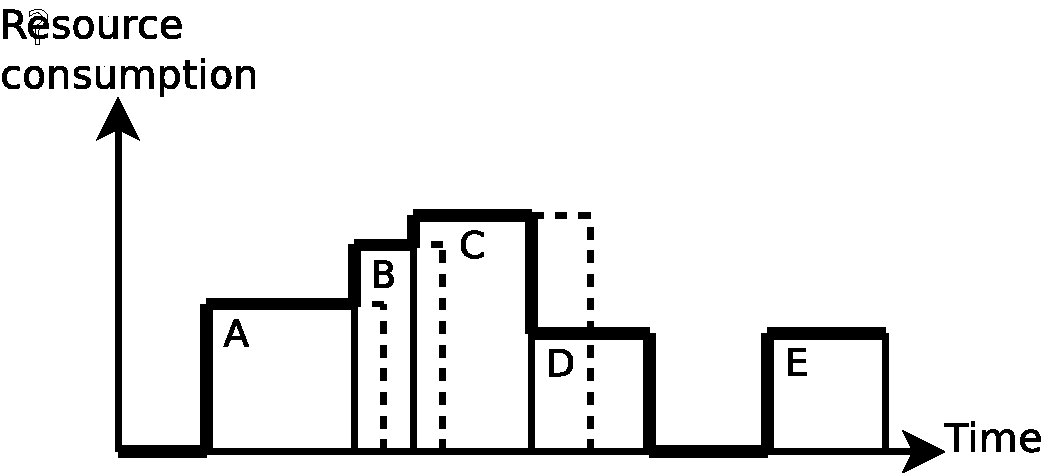
\includegraphics[width=12cm]{figures/consumptionprogress}
    \caption{As time progress, new records can invalidate old records by
    overlapping them in time. A record is depicted by a square. The stippled
    lines show where records have been invalidated. The fat line marks the
    resource consumption.}
    \label{fig:consumptionprogress}
  \end{center}
\end{figure}

% explain overlap and invalidation
On the figure it can be seen how resource consumption changes as new records
come into the system, and how old records are invalidated. Note that at one
duration there are no valid records present, which means no resource
consumption can be assumed.

% how to deal with ovarlap
As records can overlap in time, they cannot simply be summed together in order
to identity total resource consumption. Hence to know how many resources have
been consumed, one must ask for a certain point in time, where after the valid
records can be found and aggregated if needed. When there are multiple valid
records for a given point in time, the newest should be chosen. To find the
resource consumption in a time interval (e.g., for graphing resource
consumption) a set of timestamps should be generated for the interval; where
after the resource consumption can be found for each timestamp.

% how do we expect the overlap to look in the real world
Most installations will probably generate the records at a regular interval,
which will have fairly minimal overlap. However a site could also choose to
create records with very long longevity and only create new records when
resource consumption change significantly, hence taking a lazy approach to
generating storage records. Service consuming storage records must of course be
able to deal with both cases.

% several records per resource
The task of identifying overlapping records are further complicated by the fact
the a resource can generate multiple records for different parts of the
resource or splitting the resource consumption per user or group. A way to
visualize this, would be to stack several records on top of each other. In such
cases - which is likely to be the common - the task of selecting which records
are valid and which are not becomes slightly more complex. Here there will be
several records which are valid at the same time for the same resource. However
records will only be overlapping if they describe the same consumption.

% introducing 
To solve the problem of identifying if multiple record describes the same
resource consumption, the concept of consumption identity is introduced. Note
that this concept is not directly modelled into the record, but instead
something that is created from multiple properties in the record. This
consumption identity is composed of the resource identity and the subject
identity. The subject identity is defined by the SubjectIdentity property
(which can contain a number of properties). The resource identity is defined by
composing the following properties: StorageSystem, StorageShare, StorageMedia,
and StorageClass. Note that not all of these are necessarily defined, i.e., an
implicit null value. This is perfectly valid.


\subsection{Aggregating Records}

% joing consumption identity and overlapping
Having established a method to identity if two records are describing the same
consumption, it becomes possible to choose the set of currently valid records,
while ensuring that no overlapping records exists. This means that is also
becomes possible to aggregate records across storage shares, media, users,
projects in order to identify resource consumption in various contexts. For
such aggregations to make sense it is important that records are created in
a non-overlapping fashion. This is highly recommended, but not dictated by
this format specification.

% implementation suggestions
When implementing a record consuming service, it is highly recommended that a
good abstraction for choosing valid records from a given point in time, and use
this as a basis for all queries. Without such an abstraction, extracting
anything but the simplest data can become difficult. For relational database,
such an abstraction could be a set-returning function, which takes a timestamp
as its argument.

